\section{Status of the EMC effect}

One of the best tools available for studying the internal structure of nucleons is the deep inelastic
scattering (DIS) process, where a charged lepton scatters inelastically with a large four-momentum
transfer, $q^\mu$, represented by the Lorentz invariant $Q^2 = -q^\mu q_\mu \gg 1-2~\mathrm{GeV}^2$.
The process is characterized by a scaling variable Bjorken-x, $x = Q^2/2M_N \nu$, 
where $M_N$ is the mass of the target hadron and $\nu$ is the energy transferred from the lepton in the laboratory frame,
which is associated with the momentum fraction carried by a struck spin-1/2 partons in the limit of the infinite-momentum frame.
To leading order the unpolarized electromagnetic DIS cross section in the laboratory frame can be written~\cite{PhysRevD.98.030001}
\begin{equation}
    \frac{d^2 \sigma}{dx dy} = \frac{4 \pi \alpha^2}{x y Q^2} \left[ (1-y)F_2(x, Q^2) + y^2 x F_1(x, Q^2) \right]
\end{equation}
where $y = \nu/E$ where $E$ is the incident lepton energy, $\alpha$ is the fine structure constant and $F_2$
and $F_1$ are structure functions of the proton to be determined.  These structure functions can be reduced
by the Callan-Gross relation $F_2 - 2xF_1 = F_\mathrm{L} \approx 0$ for non-interacting point-like spin-1/2
particles with
\begin{equation}
    F_2(x,Q^2) = x \sum_{q} e_q^2 q(x,Q^2)
\end{equation}
where the sum $q$ is over all quark flavors,  $e_q$ is the electromagnetic chare of the quark, and the
functions $q(x,Q^2)$ are the parton distribution functions (PDFs) which are believed to be universal
and can describe other processes such as Drell-Yan scattering.  Analogous distributions exist for the case of polarized
targets.  A great success of QCD is the prediction of the logarithmic 
evolution of the PDFs with $Q^2$, the so-called DGLAP evolution.  These PDFs can in principle be measured for any bound hadronic state.

\begin{figure}[tbp]
  \centering\includegraphics[width=\columnwidth]{emc_cu_fe-crop.pdf}
  \caption{EMC effect for iron (BCDMS collaboration~\cite{Benvenuti:1987az} and SLAC E139~\cite{Gomez:1993ri})
    and copper (EMC collaboration~\cite{Ashman:1992kv}).
    Figure from Ref.~\cite{Guzey:2012yk}}
  \label{fig:emc_iron}
\end{figure}

The EMC effect~\cite{Aubert:1983xm} is the observation that the PDFs for nuclei are different than
the incoherent sum over the PDFs of the constituent nucleons and marks a clear sign of the modification
of the structure of the nucleons when bound together in a nucleus.
Since the original discovery in 1983, there has been a large
program of measurements at several laboratories, such as CERN, Fermilab, SLAC, DESY, and Jefferson Lab (JLab),
aimed at understanding the properties and probing the origin of the nuclear dependence of inelastic
structure functions (see~\cite{Geesaman:1995yd, Malace:2014uea, Hen:2016kwk} for reviews related to the EMC effect).
Measurements with high energy (of scale 100 GeV) muon beams have provided high-precision data at low to
moderate $x$ ($<0.3$), while more modest energy electron facilities (of scale 10 GeV) have provided
the highest precision at large $x$ ($>0.3$), Fig.~\ref{fig:emc_iron}.  The low-to-moderate $x$
regions show interesting shadowing and anti-shadowing behaviors, while the suppression of the
per-nucleon cross section for $0.3<x<0.7$ is the hallmark of the EMC effect.

The most comprehensive data sets with high precision at large $x$ come from SLAC E139~\cite{Gomez:1993ri} and Jlab E03-103~\cite{Seely:2009gt}. The SLAC experiment
measured the EMC effect for a wide range of nuclei, from $^4$He to Au with good precision up to
$x\approx0.8$.  One of the outcomes of E139 was an investigation of the detailed nuclear dependence of the EMC
effect. It was found that the nuclear dependence of the EMC effect at large $x$ ($x=0.6$) is consistent
with both a logarithmic $A$ dependence or a linear dependence on average nuclear density (often parametrized as an $A^{1/3}$ dependence).

The SLAC and early high energy measurements showed a number of global properties of the EMC effect:
\begin{enumerate}
 \item{The shape of the EMC effect (shadowing, anti-shadowing, and EMC regions at small, moderate, and
  large $x$ respectively) is universal and observed in all nuclei.}
 \item{The EMC effect displays little $Q^2$ dependence over the full $x$ range.}
 \item{At large $x$, the EMC effect grows with $A$, while there is little apparent $A$ dependence in the
   anti-shadowing region.}
\end{enumerate}

%%%theory
Since the first observation of the EMC effect, many theoretical models have been proposed and can be subdivided into two categories.  One includes only ``traditional'' nuclear physics effects, using convolution models with binding effects, detailed models of the nucleon momentum distribution, or pion-exchange contributions. The other category invokes more exotic explanations such as re-scaling of quark distributions in the nuclear environment, contributions of six or nine
quark bags, or modification of the internal structure of the nucleons such as ``nucleon swelling'' or suppression of point-like nucleon configurations. Several reviews give an overview of models of the EMC effect~\cite{Geesaman:1995yd, Norton:2003cb, Piller:1999wx, Hen:2013oha, Malace:2014uea}.



\subsection{EMC effect results from Jefferson Lab and the EMC-SRC correspondence}

The primary goal of Jefferson Lab E03-103 was to augment the results obtained from SLAC E139 by taking
advantage of improved target technologies to provide higher precision data for $^4$He, and the first
measurement of the EMC effect from $^3$He at large $x$.  Additional light (Be and C) and heavy (Cu and Au)
targets were also used to provide improved precision at large $x$.

Since the shape of the EMC effect is universal, the E03-103 analysis defined the ``size'' of the EMC
effect as the slope of a line fit between $0.35<x<0.7$.  This definition reduces sensitivity to
normalization uncertainties and results in higher sensitivity to the nuclear dependence.

The slope of the EMC effect for $^3$He, $^4$He, Be, and C from E03-103 plotted against scaled nuclear
density is shown in Fig.~\ref{fig:emc_jlab_hallc}.  The nuclear dependence was found to be consistent
with a simple density dependence, with the exception of $^9$Be,  which showed an anomalously larger-than-expected EMC effect given it's low average nuclear density.  However, if one considers the fact that a
beryllium nucleus can be described as two $\alpha$ clusters with an extra neutron, it then makes sense
that the EMC effect for beryllium would be more similar to $^4$He if the size of the EMC effect is
governed by the local nuclear density experienced by the quarks in the bound nucleon, rather than the
average density~\cite{Seely:2009gt, PhysRevC.82.054614}.

\begin{figure}[tbp]
  \centering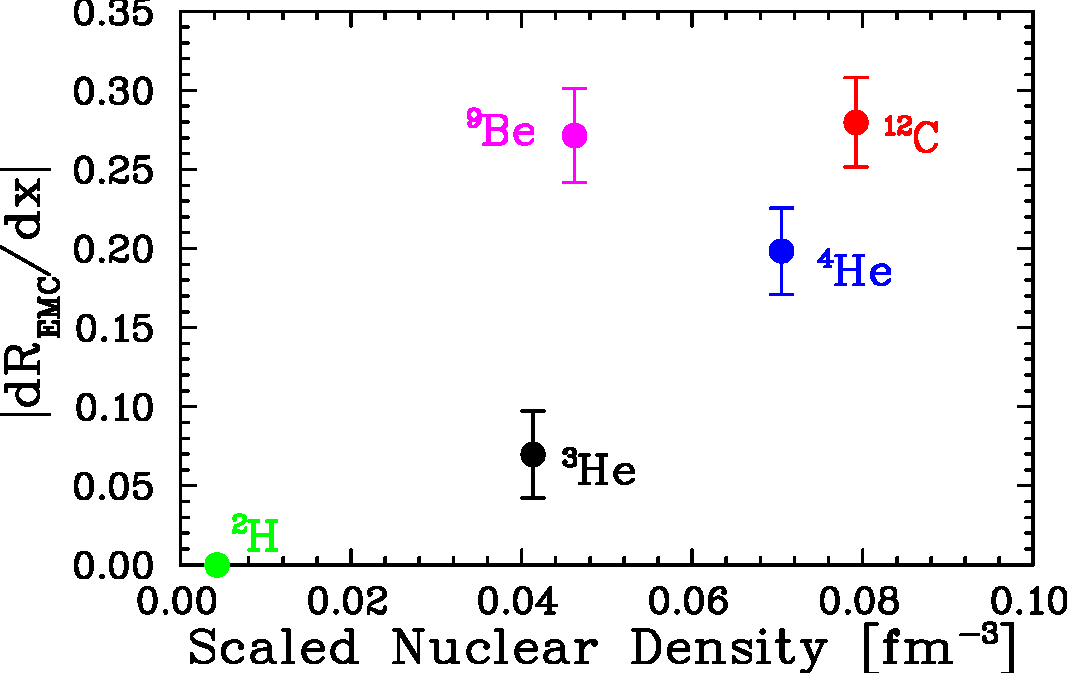
\includegraphics[width=\columnwidth]{plots/e03103_slopes.pdf}
  \caption{Size of the EMC effect (defined as $|dR/dx|$ between for $x=0.35-0.7$) vs. scaled nuclear
    density.  Figure from~\cite{Seely:2009gt}.}
  \label{fig:emc_jlab_hallc}
\end{figure}

A comparison to the $a_2=\sigma_A/\sigma_D$ ratio of
inclusive cross sections at $x>1$ (which is sensitive to the ``number of short range correlations''
found in a nucleus) a linear correlation between the two quantities was observed~\cite{Weinstein:2010rt}.
This correspondence was even more compelling when $x>1$ ratios for Be from JLab experiment E02-019 became
available and the same correlation persisted~\cite{Arrington:2012ax, Hen:2012fm}, Fig.~\ref{fig:emc_src_bff}.

\begin{figure}[tbp]
  \centering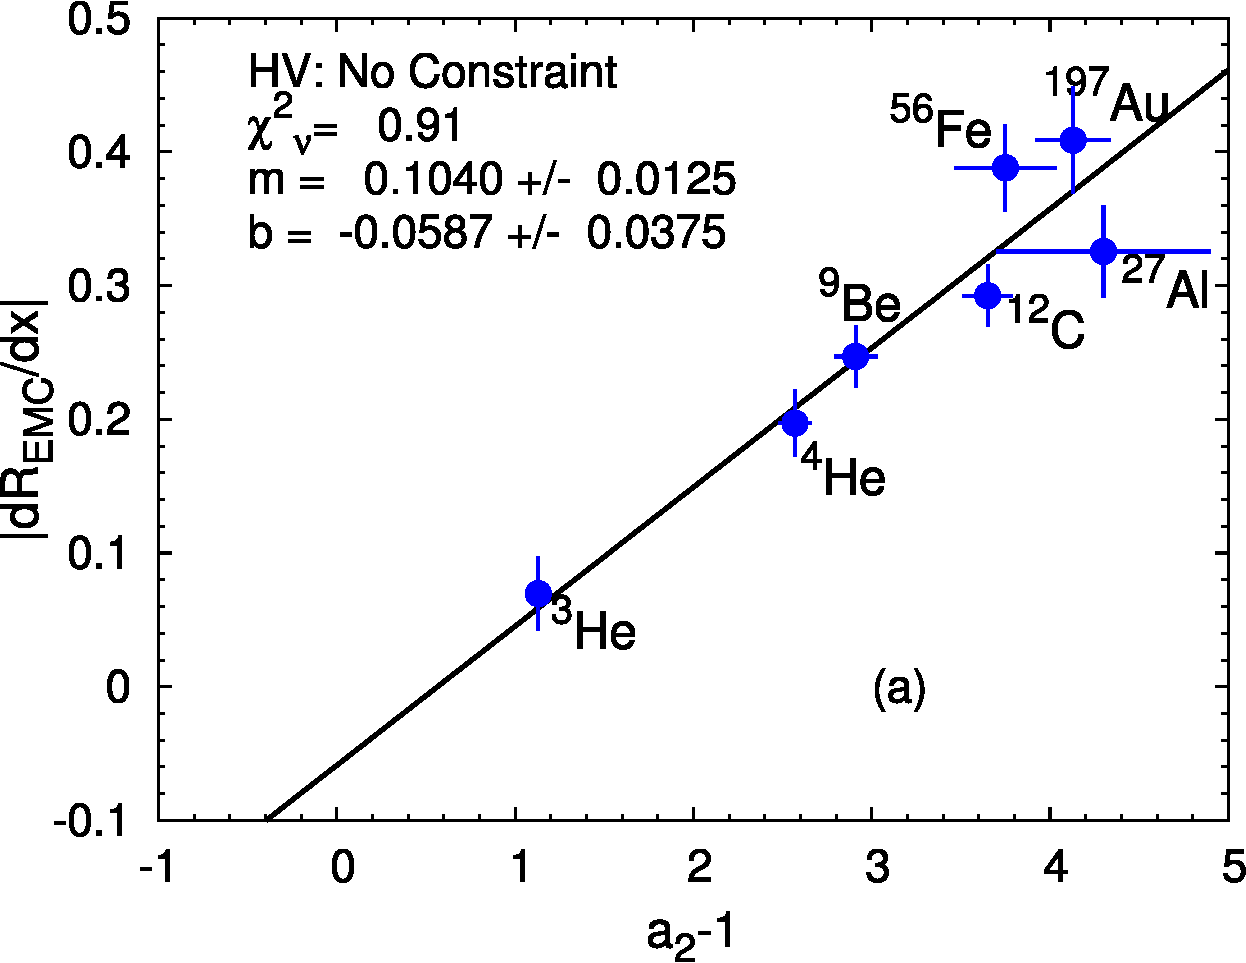
\includegraphics[width=\columnwidth]{plots/plotfit_all_norescaling_nocm_rean_final.pdf}
  \caption{Size of the EMC effect plotted vs. the SRC $a_2$ ratio. Data are from JLab and SLAC. Figure
  from Ref.~\cite{Arrington:2012ax}.}
  \label{fig:emc_src_bff}
\end{figure}

The origin of this correspondence is unclear, whether SRCs in some way cause the EMC effect, or if the two
phenomena are caused by some common underlying source.  A study was conducted to examine whether
both the EMC effect and SRCs are correlated with some other independent variable~\cite{Arrington:2012ax} such
as average nucleon separation energy, etc., with no clear common origin or factor found.

A subtlety exists in correlation studies between $x>1$ inclusive cross section ratios and the EMC effect.  The former represent the relative number of high-momentum nucleons found in an $A$ nucleus, relative to $A=2$, and not the relative number of nucleon-nucleon pairs.  This means that a causal relationsip between high-virtuality nucleons and the EMC effect can potentially represent a different scenario than one where the high-density configurations (SRC pairs) are the culprit.  Additionally, observed $NP$ dominance in SRC experiments~\cite{Subedi:2008zz} implies that for the virtuality hypotehsis, the EMC effect may differ for protons and neutrons for non-isoscalar nuclei.  Upcoming experiments at Jefferson Lab will look for signatures of such a dependence. 
\section{Quarks at $x>$1}
Quasielastic kinematics at $x>$1 probe moving nucleons, but if we increase the Q$^2$, the inelastic contribution begins to dominate, allowing us to access quark distributions. Existing JLab data have a limited range in $x$ and require the application of the of so-called "target-mass corrections" (TMCs) to extract the Q$^2\rightarrow\infty$ structure function limit.  This analysis was done for the E02-019 data, showing that the data are approaching the scaling regime~\cite{Fomin:2010ei}.  Upcoming measurements at higher energies~\cite{12gev_xgt1} can shed light on the quark structure of SRCs, where potential 6-quark configurations would result in a noticeable enhancement of the measured cross sections at $x>1$, and can be related back to the EMC region, where the enhancement is harder to determine.  Fig.~\ref{fig:quarkbags} from Ref.~\cite{Arrington:2003qt} shows the potential effect on the quark distributions in the EMC as well as the $x>1$ region.
\begin{figure}[tbp]
  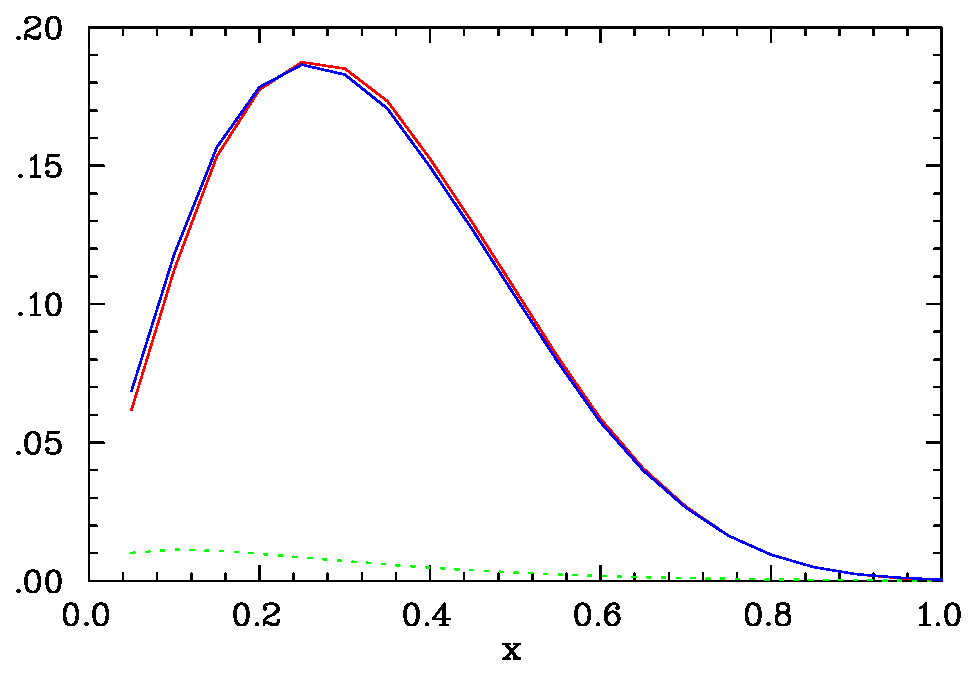
\includegraphics[width=0.45\columnwidth]{plots/qofx2_lin_5per.eps}
  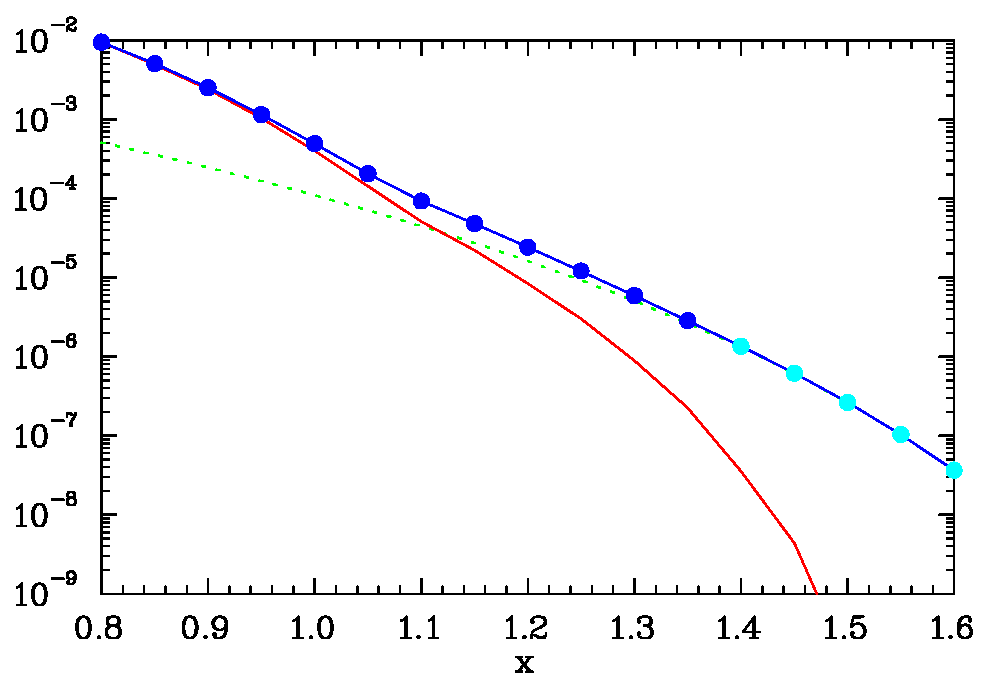
\includegraphics[width=0.45\columnwidth]{plots/qofx2_log_5per.eps}
  \caption{Quark distribution calculations for the deuteron, where the dashed line shows 2N components, the dotted line corresponds to a 5\% contribution from 6-quark bags, and the solid blue line shows the sum of the two~\cite{Mulders:1983au}. }
  \label{fig:quarkbags}
\end{figure}

